\documentclass[12pt, twoside]{article}
\usepackage[letterpaper, margin=1in, headsep=0.5in]{geometry}
\usepackage[english]{babel}
\usepackage[utf8]{inputenc}
\usepackage{amsmath}
\usepackage{amsfonts}
\usepackage{amssymb}
\usepackage{tikz}
\usetikzlibrary{quotes, angles}
\usepackage{graphicx}
\usepackage{multicol}

%\usepackage{pgfplots}
%\pgfplotsset{width=10cm,compat=1.9}
%\usepgfplotslibrary{statistics}
%\usepackage{pgfplotstable}
%\usepackage{tkz-fct}
%\usepackage{venndiagram}

\usepackage{fancyhdr}
\pagestyle{fancy}
\fancyhf{}
\renewcommand{\headrulewidth}{0pt} % disable the underline of the header

\fancyhead[RE]{\thepage}
\fancyhead[RO]{\thepage \\ Name: \hspace{3cm}}
\fancyhead[L]{BECA / Dr. Huson / Geometry 10th Grade\\* Unit 4: Parallels and transversals \\ 23 October 2019}

\begin{document}
\subsubsection*{4.4 Do Now: Area, volume, perimeter}
  \vspace{0.25cm}
  \begin{enumerate}


  \item Given the rectangle $ABCD$ shown below, with length $16$ and width $7$. Find the figure's area.
  \begin{flushright}
  \begin{tikzpicture}[scale=1]
    \draw [-, thick] (0,0)--(6,0)--(6,3)--(0,3)--cycle;
    \draw [fill] (0,0) circle [radius=0.05] node[left]{$A$};
    \draw [fill] (6,0) circle [radius=0.05] node[right]{$B$};
    \draw [fill] (6,3) circle [radius=0.05] node[right]{$C$};
    \draw [fill] (0,3) circle [radius=0.05] node[left]{$D$};
    \node at (6.5, 1.5){$7$};
    \node at (3, -0.5){16};
  \end{tikzpicture}
  \end{flushright}
  \vspace{1.5cm}

\item The area of a rectangle is 51 square inches and one side is $4.25$ inches high. What is its other dimension, the length?
\begin{flushright}
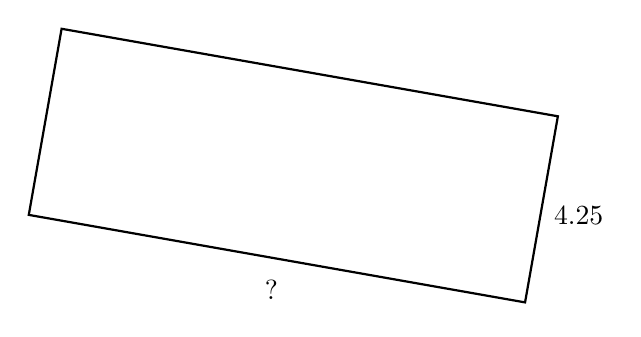
\begin{tikzpicture}[scale=0.8, rotate=-10]
  \draw [-, thick] (0,0)--(8,0)--(8,3)--(0,3)--cycle;
  \node at (8.6, 1.5){$4.25$};
  \node at (4, -0.5){?};
\end{tikzpicture}
\end{flushright}
\vspace{1.5cm}

\item Draw a square that has an area of 16 square centimeters. Label its sides with their length and state the length of the square's perimeter.

\newpage

\item Find the area of the parallelogram $BECA$ shown below, with base $BE=6.75$ and height $h=3.8$.
\begin{flushright}
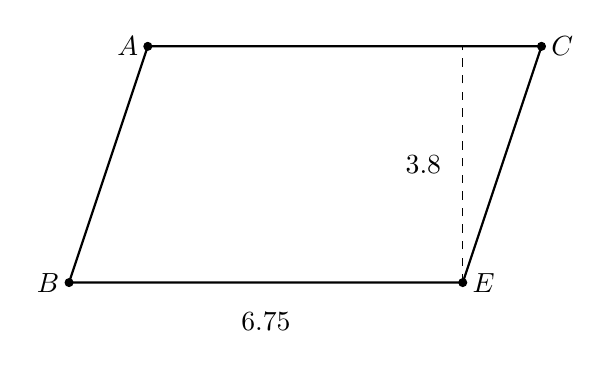
\begin{tikzpicture}[scale=1]
  \draw [-, thick] (0,0)--(5,0)--(6,3)--(1,3)--cycle;
  \draw [-, dashed] (5,0)--(5,3);
  \draw [fill] (0,0) circle [radius=0.05] node[left]{$B$};
  \draw [fill] (5,0) circle [radius=0.05] node[right]{$E$};
  \draw [fill] (6,3) circle [radius=0.05] node[right]{$C$};
  \draw [fill] (1,3) circle [radius=0.05] node[left]{$A$};
  \node at (4.5, 1.5){$3.8$};
  \node at (2.5, -0.5){6.75};
\end{tikzpicture}
\end{flushright}

\item The area of the parallelogram shown below is 49.5 sq. cm. (not drawn to scale). Its longer sides are 9 cm long. Find the length of a perpendicular between the two longer sides, $h$.
\begin{flushright}
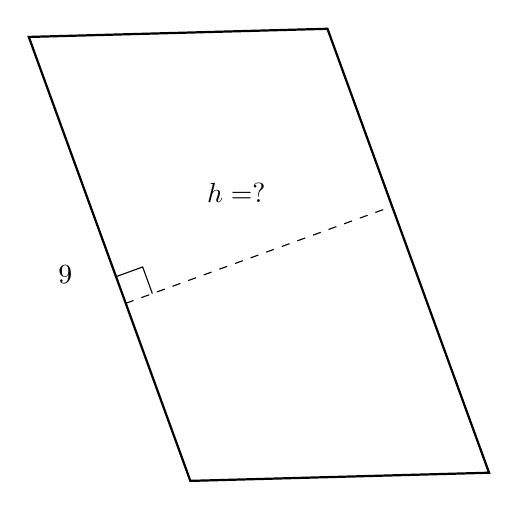
\begin{tikzpicture}[scale=1.2, rotate=-70]
  \draw [-, thick] (0,0)--(5,0)--(6,3)--(1,3)--cycle;
  \draw [-, dashed] (3,0)--(3,3);
  \draw (3,0)++(-0.3,0)--++(0,0.3)--+(0.3,0);
  \node at (2.3, 1.5){$h=?$};
  \node at (2.5, -0.5){9};
\end{tikzpicture}
\end{flushright}

\item Find the volume of a box (rectanglar prism) having a length of 8 centimeters, a depth of 4 cm, and a height of 5 cm. Show the calculation.
\begin{flushright}
  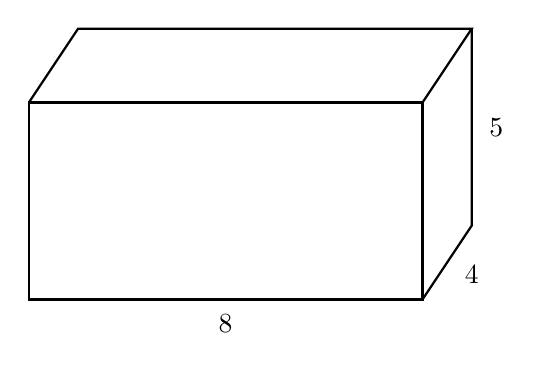
\begin{tikzpicture}[scale=1.25]
    \draw [-, thick] (0,0)--(4,0)--(4,2)--(0,2)--cycle;
    \draw [-, thick] (0,2)--(0.5,2.75)--(4.5,2.75)--(4,2);
    \draw [-, thick] (4,0)--(4.5,0.75)--(4.5,2.75);
    \node at (4.75, 1.75){$5$};
    \node at (2, -0.25){$8$};
    \node at (4.5, 0.25){$4$};
  \end{tikzpicture}
  \end{flushright} \vspace{2cm}
  
\newpage 


\item  A cardboard mailing carton is $10 \frac{1}{2}$ inches long, 7 inches wide, and $1 \frac{1}{2}$ inches tall. Find the volume of the box. Show the calculation.
  \begin{flushright}
    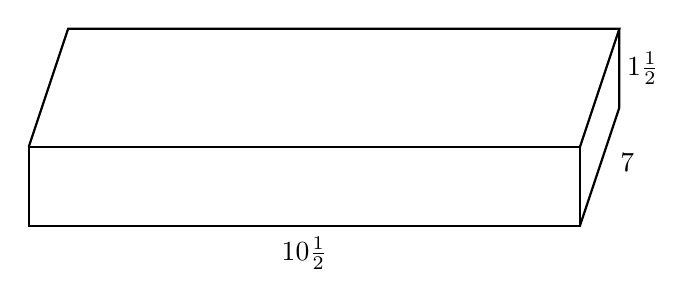
\begin{tikzpicture}[scale=1]
      \draw [-, thick] (0,0)--(7,0)--(7,1)--(0,1)--cycle;
      \draw [-, thick] (0,1)--(0.5,2.5)--(7.5,2.5)--(7,1);
      \draw [-, thick] (7,0)--(7.5,1.5)--(7.5,2.5);
      \node at (7.8, 2){$1 \frac{1}{2}$};
      \node at (3.5, -0.35){$10 \frac{1}{2}$};
      \node at (7.6, 0.8){$7$};
    \end{tikzpicture}
    \end{flushright} \vspace{2cm}

\item  Find the volume of a packing crate  $32$ inches long, 10 inches wide, and $1$ foot tall. Show the calculation.
\begin{flushright}
  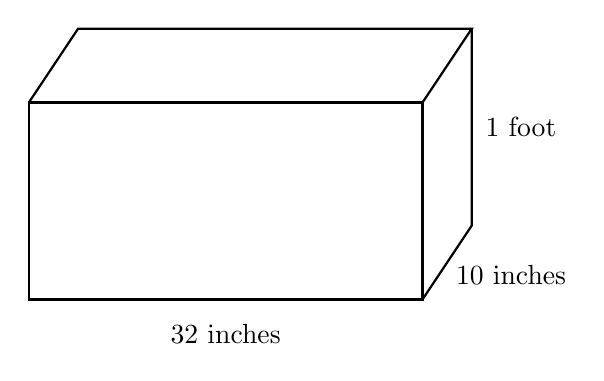
\begin{tikzpicture}[scale=1.25]
    \draw [-, thick] (0,0)--(4,0)--(4,2)--(0,2)--cycle;
    \draw [-, thick] (0,2)--(0.5,2.75)--(4.5,2.75)--(4,2);
    \draw [-, thick] (4,0)--(4.5,0.75)--(4.5,2.75);
    \node at (5.0, 1.75){$1$ foot};
    \node at (2, -0.35){$32$ inches};
    \node at (4.9, 0.25){$10$ inches};
  \end{tikzpicture}
  \end{flushright} \vspace{1cm}


\item A wooden post laying on the ground is 200 centimeters long. The post's cross section is square. If its volume is 12,800 cubic centimeters, what is the dimension of each side of its square end, $x$? (not to scale)
\begin{flushright}
  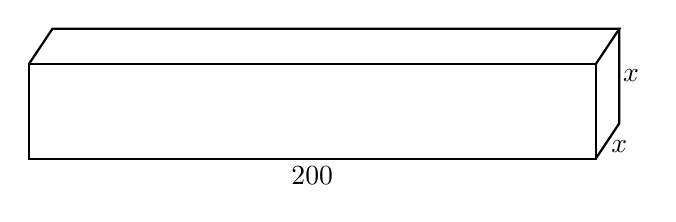
\begin{tikzpicture}[scale=.6]
    \draw [-, thick] (0,0)--(12,0)--(12,2)--(0,2)--cycle;
    \draw [-, thick] (0,2)--(0.5,2.75)--(12.5,2.75)--(12,2);
    \draw [-, thick] (12,0)--(12.5,0.75)--(12.5,2.75);
    \node at (12.75, 1.75){$x$};
    \node at (6, -0.35){$200$};
    \node at (12.5, 0.25){$x$};
  \end{tikzpicture}
  \end{flushright} \vspace{2cm}

\newpage 

\item Find the area of $\triangle CAT$. The altitude $h$ of the triangle is 6.7 centimeters and the base $CA=13.1$ cm. Show work by writing an equation before making the calculation. \\[0.5cm]
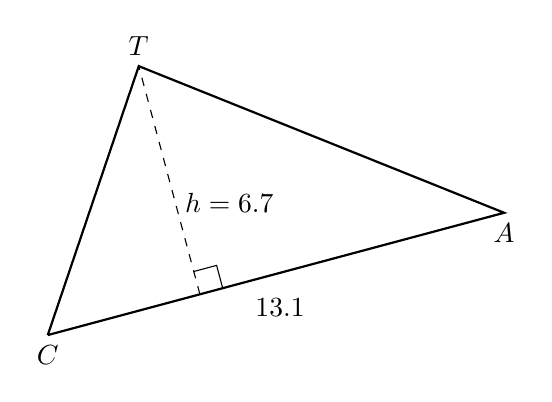
\begin{tikzpicture}[scale=1, rotate=15]
  \draw [thick]
    (2,0)node[below]{$C$}--
    (8,0)node[below]{$A$}--
    (4,3)node[above]{$T$} --(2,0);
 \draw [dashed] (4,0)--(4,3);
 \draw (4,0)++(0.3,0)--++(0,0.3)--+(-0.3,0);
 \node at (4,1.2)[right]{$h=6.7$};
 \node at (5,-0.2)[below]{$13.1$};
\end{tikzpicture} \vspace{1.0cm}


\item The side $\overline{AB}$ of triangle $ABC$ is extended and an altitude to the vertex $C$ is drawn, as shown below. The triangle's height is $h=7.25$ and its base measures $AB=12.4$. Find the area of the triangle.\\[0.25cm]
   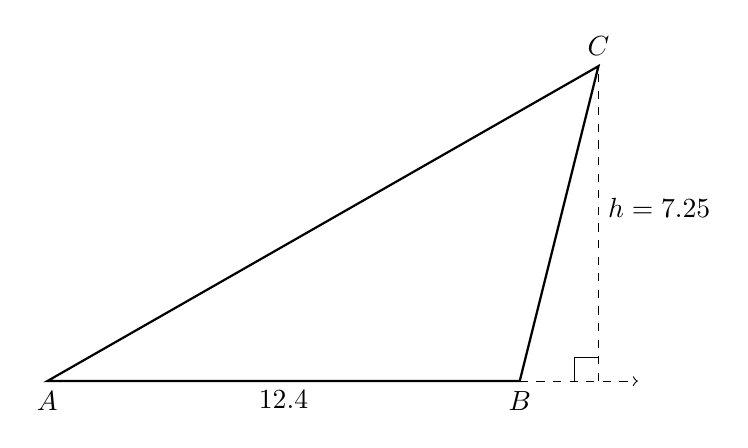
\begin{tikzpicture}[scale=1]
     \draw [thick]
       (0,0)node[below]{$A$}--
       (6,0)node[below]{$B$}--
       (7,4)node[above]{$C$} --cycle;
    \draw [dashed] (7,0)--(7,4);
    \draw [dashed, ->] (6,0)--(7.5,0);
    \draw (7,0)++(-0.3,0)--++(0,0.3)--+(0.3,0);
    \node at (7,2.2)[right]{$h=7.25$};
    \node at (3,0)[below]{$12.4$};
  \end{tikzpicture} \vspace{1.0cm}
  

\item One side of the $\triangle ABC$ has a length $AB=16$. The triangle's area is 96. Find the length of the altitude $h$ of the triangle to vertex $C$ and perpendicular to side $\overline{AB}$.\\[0.5cm]
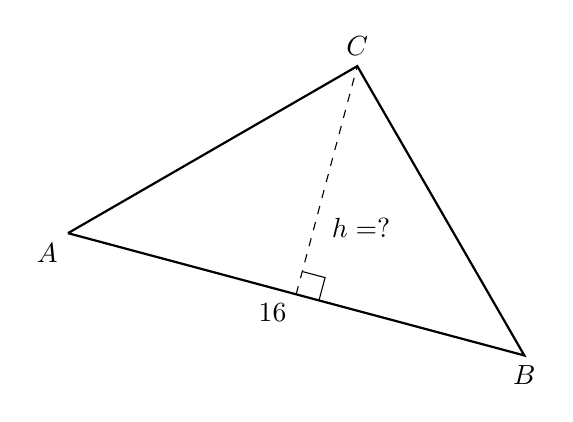
\begin{tikzpicture}[scale=1, rotate=-15]
\draw [thick]
  (2,0)node[below left]{$A$}--
  (8,0)node[below]{$B$}--
  (5,3)node[above]{$C$} --(2,0);
\draw [dashed] (5,0)--(5,3);
\draw (5,0)++(0.3,0)--++(0,0.3)--+(-0.3,0);
\node at (5.1,0.9)[right]{$h=?$};
\node at (5,0)[below left]{$16$};
\end{tikzpicture} \vspace{1.0cm}

\item The shape shown below is composed of straight lines and right angles, with some lengths as marked. Find the area of the figure. (the figure is not drawn to scale)
\begin{flushleft}
\begin{tikzpicture}[scale=0.5]
  \draw [-, thick] (0,0)--(13,0)--(13,3)--(9,3)--(9,9)--
  (0,9)--(0,7)--(4,7)--(4,3)--(0,3)--cycle;
  %\draw [fill] (0,0) circle [radius=0.05] node[left]{$A$};
  %\draw [fill] (7,0) circle [radius=0.05] node[right]{$B$};
  %\draw [fill] (7,2) circle [radius=0.05] node[right]{$C$};
  %\draw [fill] (0,2) circle [radius=0.05] node[left]{$D$};
  \node at (4.5, 5){3};
  \node at (2, 2.5){3};
  \node at (8.5, 5){5};
  \node at (11, 2.5){3};
  \node at (6.5, -0.5){10};
  \node at (13.5, 1.5){2};
  %\node at (13.5, 8){2};
\end{tikzpicture}
\end{flushleft} \vspace{2cm}

\item The volume of the rectanglar prism shown is 105 cubic meters. Its length is 7.5 meters and depth 4 m. Find its height $h$. Show the calculation. (not drawn to scale)
\begin{flushright}
  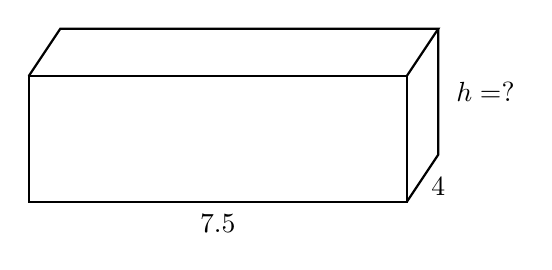
\begin{tikzpicture}[scale=0.8]
    \draw [-, thick] (0,0)--(6,0)--(6,2)--(0,2)--cycle;
    \draw [-, thick] (0,2)--(0.5,2.75)--(6.5,2.75)--(6,2);
    \draw [-, thick] (6,0)--(6.5,0.75)--(6.5,2.75);
    \node at (7.25, 1.75){$h=?$};
    \node at (3, -0.35){$7.5$};
    \node at (6.5, 0.25){$4$};
  \end{tikzpicture}
  \end{flushright} \vspace{1cm} 

  \item The shape shown below is a trapezoid. Its height is 3.2 cm and the longer base is 6.0 cm. The shorter side opposite the base is 4.8 cm. \\[0.25cm]
  Find the area of the figure.
  \begin{flushright} 
  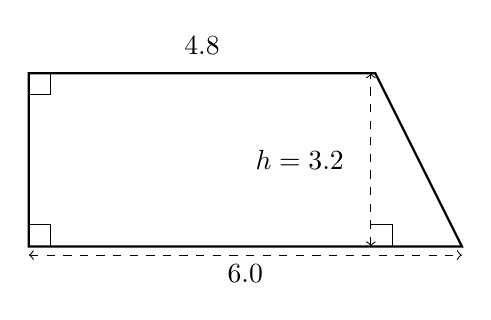
\begin{tikzpicture}[scale=1.1]
    \draw [thick]
    (3,0)--(3,2)--(7,2)--(8,0)--cycle;
    \draw [dashed,<->] (6.95,0)--(6.95,2);
    %\draw [dashed,<->] (0,2.1)--(7,2.1);
    %\draw [->] (45:0.5)--(45:0.9142);
    %\draw [->] (45:2.3)--(45:1.9142);
    \draw (3,0)++(0,0.25)--++(0.25,0)--+(0,-0.25);
    \draw (3,2)++(0,-0.25)--++(0.25,0)--+(0,0.25);
    \draw (6.95,0)++(0,0.25)--++(0.25,0)--+(0,-0.25);
    \draw [dashed,<->] (3,-0.1)--(8,-0.1);
    \node at (5.5,-0.1)[below]{$6.0$};
    \node at (6.75,1)[left]{$h=3.2$};
    \node at (5,2.1)[above]{$4.8$};
  \end{tikzpicture}
  \end{flushright} 
  \vspace{4cm}


 
  \item A rectangle has two triangular cutouts as shown with lengths marked. Find the area of the figure. (the figure is not drawn to scale)
  \begin{flushleft}
  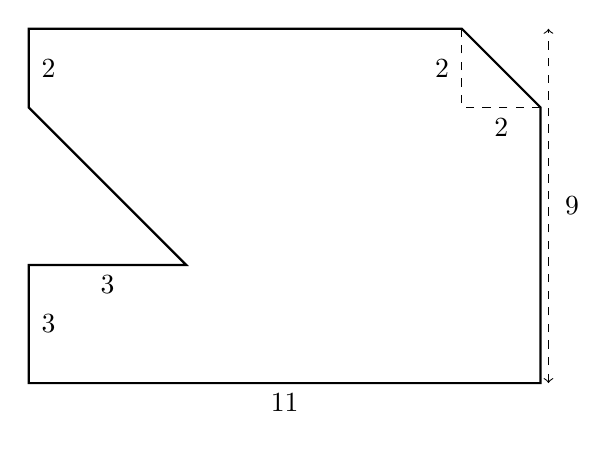
\begin{tikzpicture}[scale=0.5]
    \draw [-, thick] (0,0)--(13,0)--(13,7)--(11,9)--
    (0,9)--(0,7)--(4,3)--(0,3)--cycle;
    \draw [dashed] (13,7)--(11,7)--(11,9);
    \draw [<->, dashed] (13.2,0)--(13.2,9);
    %\draw [fill] (0,0) circle [radius=0.05] node[left]{$A$};
    %\draw [fill] (7,0) circle [radius=0.05] node[right]{$B$};
    %\draw [fill] (7,2) circle [radius=0.05] node[right]{$C$};
    %\draw [fill] (0,2) circle [radius=0.05] node[left]{$D$};
    \node at (0.5, 8){2};
    \node at (0.5, 1.5){3};
    \node at (2, 2.5){3};
    \node at (10.5, 8){2};
    \node at (12, 6.5){2};
    \node at (6.5, -0.5){11};
    \node at (13.8, 4.5){9};
    %\node at (13.5, 8){2};
  \end{tikzpicture}
  \end{flushleft} \vspace{2cm}

  \item The length of the given rectangle is 10 more than the width. Its area is 75. Find the length and width of the rectangle using an algebraic method.\\[5pt]
  (the drawing is not to scale)
  \begin{flushright}
  \begin{tikzpicture}
    \draw [-, thick] (0,0)--(4.5,0)--(4.5,2)--(0,2)--cycle;
    \node at (5, 1){x};
    \node at (2.25, -0.5){$x+10$};
  \end{tikzpicture}
  \end{flushright} \vspace{5cm}

  \end{enumerate}
\end{document}
